%\section{Аналитическая часть}

%\subsection{Формализация задачи}
В соответствии с темой необходимо разработать метод, позволяющий по нечёткому описанию на русском языке определить объект, принадлежащий готовой ограниченной выборке. 

В рамках поставленной задачи в качестве выборки используются понятия из словаря терминов в области ДВС \cite{ICE}, список выбранных слов указан в приложении A. Для того, чтобы обеспечить работоспособность метода, необходимо заранее собрать как можно больше определений выбранных терминов.

На вход подаётся словесное описание какого-либо термина из этого набора. Оно представляется в виде множества слов, связанных между собой по смыслу и грамматически, на русском языке. 

Результатом является термин, заданное описание которого наиболее совпадает с введённым. Термин представляет из себя одно слово или словосочетание. 

Для выполнения данной задачи требуется выполнить следующие шаги:
\begin{enumerate}
	\item предварительно подготовить терминологическую базу знаний, в основе которой лежат сущности конкретной предметной области и их множественные определения;
	
	\item полученное входное описание сравнить с имеющимися в базе знаний;
	
	\item по результатам сравнения выбрать наиболее подходящий термин. \newline
\end{enumerate}

\subsection{Возможные области применения}
Подобный метод может быть применён в медицинских системах, ориентированных на определение вида заболевания с последующим подбором наиболее целесообразного способа лечения по описанию симптомов, результатов обследований и т.д. 

Также он может быть привлечён в системах контроля и оценки знаний учащихся, в частности, в заданиях с развёрнутым ответом, для оценивания правильности которого привлекаются специалисты. Разрабатываемый подход может позволить освободить часть сотрудников от этой работы, и снизить роль человеческого фактора. О необходимости снижения которого не раз заявляли руководители Федеральной службы по надзору в сфере образования и науки. Снижение этого показателя стало одной из причин создания ЕСОКО (единая система оценки качества образования).

Кроме того, метод может быть полезен при повышении квалификации или переквалификации работников, поскольку в любой сфере деятельности \, складывается определённая динамическая система понятий, термины которой далеко не всегда могут быть общеизвестными, особенно, это касается узких специальностей. Рассматриваемый метод помогает решить подобную проблему, позволяя по введённому описанию определить термин, который с наибольшей вероятностью имелся в виду.

Также он может быть внедрён в системы поиска документов по формальному описанию их содержимого. \newline

\subsection{Анализ существующих решений}
Задача определения какого-либо объекта: будь то документ или термин, по его описанию ставится практически в каждой области, предполагающей повторное использование уже накопленных данных. Для автоматизации процесса поиска разрабатываются системы, ориентированные на её решение. \\

\textbf{Autonomy}

Представляет из себя поисковую систему, предоставляющую пользователям возможность делать запросы на естественном языке. Система анализирует введённый текст, извлекает из него смысловое содержание и помещает в специальный конфигурационный файл, который привлекается в дальнейшем при поиске \cite{isystem}.

Помимо этого, в совокупности с платформой IDOL 10 стало возможным работать практически со всеми видами представления информации: аудио, видео, электронная почта, веб-контент и структурированными машинными данными (например, журналы транзакций, показатели счётчиков и др.), позволяя извлекать смысловую информацию без предварительной обработки, особенно это касается аудио- и видеофайлов \cite{autonomy_cite,autonomy}.\\
%
Такое расширение возможностей позволило создать следующие решения:
%
\begin{itemize}
	\item Autonomy Legal Hold -- сбор информации для судебных разбирательств;
	
	\item Autonomy Investigator -- поиск информации, связанной с фактами мошенничества;
	
	\item Autonomy Voice Discovery -- работа с аудиозвонками. \\
\end{itemize}

\textbf{Webcompass}

Webcompass -- поисковая система, предназначенная для специалистов (в отличие от Autonomy, которая в основном взаимодействует с конечными пользователями), которые могут структурно сформулировать свой запрос, а также промаркировать области поиска, в которых наиболее вероятно можно найти ответ \cite{isystem}.

И Autonomy, и Webcompass -- коммерческие системы, что касается исследовательских проектов, то можно привести в пример систему MARRI. \\

\textbf{MARRI}

Поскольку большой объём информации приходится на сеть Интернет, то большинство проектов ориентировано на поиск необходимых Web-страниц. К ним относится и система MARRI, обрабатывающая \, запросы определённой \, предметной области. 

Для того, чтобы решить поставленную задачу, \, используются знания, \, представленные в виде онтологий, которые в текущем проекте понимаются как множества концептов и связей между ними. 

Основная идея заключается в том, что подходящие тексты содержат фрагменты, которые могут быть сопоставимы с онтологией предметной области. Таким образом, при анализе страниц проверяется их соответствие онтологическому тесту, по результатам которого система возвращает пользователю только те страницы, которые его прошли \cite{marri}.

Краткий сравнительный анализ приведён в таблице \ref{cmp_table}.
\begin{table}[h]
	\begin{center}
		\caption{Сравнительный анализ существующих решений}
		\label{cmp_table}
		\begin{tabular}{| p{5cm} | p{3.5cm} | p{3.57cm} | p{3.1cm} |}
			\hline
			\backslashbox{\textbf{Критерий}}{\textbf{Решение}} 	& Autonomy & Webcompass	& MARRI \\
			\hline
			Возможность работы с ЕЯ 				& Есть 					& Нет 							& Есть \\ 
			\hline
			Тип обрабатываемых документов 	  		& Текстовые документы, аудио, видео, …	& Web-страницы 					& Web-страницы \\ 
			\hline
			Целевая аудитория 							& Широкая	& Узкопрофильная & Широкая \\ 
			\hline
			Стоимость						 		& Высокая 				& Нет данных 					& Нет данных \\ 
			\hline
		\end{tabular}
	\end{center}
\end{table}

\subsection{Онтология}
В основе множества современных проектов, ориентированных на работу с естественным языком (в том числе и тех, что были рассмотрены ранее) нередко положены онтологии. \\

\textbf{Понятие онтологии}

 Термин <<онтология>> заимствован из философии, где под ним подразумевается система категорий, являющихся следствием определённого взгляда на мир \cite{philosophy}.

В настоящий момент понимание этого термина различно, всё зависит от контекста и поставленной цели. Что касается информационных технологий, то в этой сфере она рассматривается как удобная абстракция для отображения накопленных знаний в некоторой предметной области \cite{isystem,gruber}.

Наиболее распространено следующее определение: <<Онтология -- это явная спецификация концептуализации>> \cite{gruber}. Под концептуализацией подразумевается упрощённый взгляд на мир, который нужно представить для достижения какой-либо цели. Как правило, онтологии включают не только общие, но и специфичные для рассматриваемой области термины. \\
%
Преимущество онтологий в том, что они позволяют \cite{ontology_guide}:
%
\begin{itemize}
	\item накапливать знания в конкретной предметной области;
	
	\item повторно их использовать (детально проработанная \, онтология может \, быть интегрирована в несколько проектов, избавляя разработчиков от \, необходимости создавать её заново);
	
	\item анализировать их (анализ имеющихся терминов особо важен как при повторном использовании, так и при их расширении);	
	
	\item совместно использовать накопленные знания конкретной области;
	
	\item явно выделить имеющиеся допущения. \newline
\end{itemize}

\textbf{Теоретико-модельная формализация}

На рисунке \ref{fig1:image} приведена общая схема моделирования системы. Как правило, моделируемая предметная область представляется в виде некоторого набора текстовых документов на естественном языке, далее на их основе строится теория предметной области, при этом особое внимание уделяется формальному описанию онтологии \cite{solution_task}.
\begin{figure}[h]
	\begin{center}
		{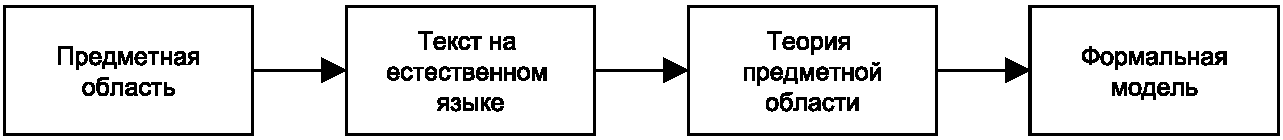
\includegraphics[scale = 0.6]{img/ontology.pdf}}
		\caption{Общая схема.}
		\label{fig1:image}
	\end{center}
\end{figure}

\newpage

\textbf{Модели онтологии}

Под формальной моделью онтологии предметной области будем называть пару
\begin{equation}\label{formula1}
	O = \left(  \sigma, A   \right),
\end{equation}
где $\sigma$ -- множество ключевых понятий предметной области, $A$ -- множество предложений, описывающих их смысл. 

Множество $\sigma$ называют сигнатурой онтологии предметной области. Множество $A$ состоит из определений символов, содержащихся в сигнатуре $\sigma$. 

Однако множество предложений может содержать сигнатурные символы, которые не являются символами ключевых понятий предметной области. Это возникает из-за того, что при их описании  использовались утверждения, в которых содержались термины другой тематики.

Онтология, которая представляется формулой (\ref{formula1}) может быть полезна при составлении спецификаций, а именно, для описания терминов, принадлежащих узкой предметной направленности \cite{solution_task}. \newline

\subsection{Особенности естественного языка}\label{sec:features_NL}
Естественный язык (ЕЯ) -- сложная многоуровневая система, которая возникла для обмена информацией в процессе практической деятельности человека, кроме того, постоянно изменяется в связи с ней \cite{lingvocabulary, auto_processing_nl}. \\
%
Возможно несколько способов разбиения текста на ЕЯ на уровни \cite{natural_lang_processing}:
%
\begin{itemize}
	\item синтаксический уровень (уровень предложений);
	
	\item морфологический уровень (уровень слов);
	
	\item фонологический уровень (уровень фонем для устной речи/уровень символов для письменный текстов).
\end{itemize}

Подобное разбиение условно, поскольку в зависимости от задачи может выделяться отдельно уровень морфем (значимая часть слова) как подуровень морфологического уровня. Также может быть выделен лексический уровень.

\subsection{Предобработка текста на ЕЯ}\label{sec:before_work}
Для достижения наилучшего качества обработки текста на ЕЯ необходимо сначала провести его предобработку, чтобы привести его в удобный для работы формат. \\
%
Предобработка может включать в себя \cite{evaluation_preprocessing}:
%
\begin{itemize}
	\item нормализацию:
	\begin{itemize}
		\item перевод всех букв в тексте в один регистр;
		
		\item удаление знаков пунктуации;
		
		\item удаление цифр/чисел или замена на текстовый эквивалент;
	\end{itemize}
	
	\item токенизацию (чаще всего по словам);
	
	\item лемматизацию (приведение слова к словарной форме -- лемме)/стемминг (процесс отбрасывания словообразующих морфем);
	
	\item удаление стоп-слов, т.е. слов, которые не несут смысловой нагрузки;
	
	\item векторизацию. \newline
\end{itemize}

\subsection{Векторизация}\label{sec:vect}
Используется для представления текста в удобном формате. Наиболее \, простой способ -- <<мешок слов>> (<<bag-of-words>>) или набор ключевых слов или терминов. При таком подходе игнорируется порядок единиц, входящих в состав рассматриваемого текста.

Под терминами коллекции документов $D$ будем понимать все одиночные слова (кроме стоп-слов), которые встретились в тексте хотя бы  в одном из документов. В итоге получается множество всех терминов коллекции:
\begin{equation}
	\tau = \, \left\lbrace t \, | \, t - \;\text{термин} \, \right\rbrace. 
\end{equation}

Каждый документ в пространстве терминов представляется в виде вектора:
\begin{equation}
	d = \left( t_1, ..., t_{|\tau|} \right)^T, \; d \in D,
\end{equation}
где каждое число -- координата вектора, соответствует конкретному термину и равняется его весу в данном документе. \newline

\subsubsection{Методы для вычисления веса слова в тексте}\label{sec:weight}
\textbf{BinaryBOW}

В самом простом, бинарном, случае такая координата принимает значение 1, если соответствующий термин встречается в документе, 0 -- иначе \cite{auto_processing_nl_cl}. \newline

\textbf{CountBOW}

Рассматривается следующий подход: чем чаще слово употреблено в тексте, тем больше его значимость. Таким образом, координата вектора фиксирует количество вхождений этого термина \cite{review}. \newline

\textbf{TF-IDF, Term Frequency -- Inverse Document Frequency}

Для того, чтобы избежать зависимости значимости термина от длины рассматриваемого документа, следует нормализовать количество его вхождений. Такая величина называется частотой термина (Term Frequency или TF).  

Метод TF-IDF предполагает, что значимость термина прямо пропорциональна частоте его появления в документе и обратно пропорциональна доле документов в наборе, в которых он употреблён.

При таком подходе наибольший вес получает тот термин, который часто встречается в одном или небольшой группе документов, но не встречается в остальных, то есть, является некой отличительной особенностью на фоне часто употребляемых слов \cite{an_information}. 

Таким образом, учитывая коллекцию документов $D$, термин $t$ и текущий документ $d \in D$, вес вычисляется по формуле (\ref{formula2}):
\begin{equation}\label{formula2}
	t(d) = f(t, d) \cdot \ln \left( \frac{\left| D \right| }{f(t, D)} \right), 
\end{equation}
где $f(t, d)$ -- количество появлений $t$ в $d$ (\ref{formula7}), $\left| D \right| $ -- число документов в коллекции, $f(t, D)$ -- количество документов, в которых встречается рассматриваемый термин (\ref{formula8}).

\begin{equation}\label{formula7}
	f(t, d) = \frac{n_t}{\sum\limits_{k}n_k},
\end{equation}
где $n_i$ -- количество появлений в рассматриваемом документе $d$ соответствующего термина $i$.

\begin{equation}\label{formula8}
	f(t, D) = \left| \{d_i \in D | t_i \in d_i\} \right|
\end{equation}

Может возникнуть несколько ситуаций в зависимости от принимаемых значений этими аргументами \cite{using_tf_idf}.

Предположим, что $\left| D \right|  \sim f(t, D)$, то есть, размер корпуса документов примерно равен количеству употреблений $t$ в $D$. Другими словами, термин $t$ употребляется в большинстве документов онтологии.
	
Если выполняется условие (\ref{formula3}):
\begin{equation}\label{formula3}
	c < \ln \left( \frac{\left| D \right| }{f(t, D)} \right) < 1,
\end{equation}
где $c$ -- константа с малым значением, то $t(d)$ будет меньше, чем $f(t, d)$.

Это означает, что $t$ широко распространён по всей коллекции документов. Чаще всего подобное поведение наблюдается в отношении очень общих слов, а также таких как союзы, предлоги, которые сами по себе, как правило, не несут ключевого значения. Подобные слова имеют очень низкое значение TF-IDF, тем самым, помечаются как незначительные при поиске.

С другой стороны, предположим, что $f(t, D)$ принимает очень малое значение (термин употреблён лишь в малом количестве документов онтологии), в то время как $f(t, d)$ очень большое (термин часто используется в пределах документа). Получается, что логарифм из формулы (\ref{formula2}) также достаточно большой по величине, что напрямую сказывается на $t(d)$. Следовательно, рассматриваемый термин имеет высокий вес, что подчёркивает его важность. В таком случае говорят, что $t$ обладает большой дискриминационной силой.

При таком подходе необходимо учитывать тот факт, что не все <<редкие>> слова могут быть важны в рамках рассматриваемой задачи. Для того, чтобы сократить множество терминов, вводится понятие частоты документов или DF (Document frequency) \cite{evaluation_preprocessing}. \newline

\textbf{Возможная модификация TF-IDF} 

Частота документов -- количество документов, в которых встречается термин. Вводится пороговое значение DF, которое в отличие от удаления стоп-слов, призванного уменьшать количество высокочастотных, не имеющих отношения к теме слов, устраняет нечастые слова. 

Все термины, встречающиеся меньше, чем в $m$ документах коллекции, не рассматриваются, где $m$ -- заранее определённый порог.

Пороговое значение DF основано на предположении, что нечастые слова не являются информативными. Если установить его в 1, то термины, которые встречаются только в одном документе, учитываться не будут. \newline

\textbf{Адаптация TF-IDF к рассматриваемой задаче}

Разрабатываемый метод строится на предположении, что, несмотря на то, что определения дают разные люди, они пересекаются в ключевых моментах. Иными словами, есть какие-либо свойства, характеристики, которые являются отличительной чертой рассматриваемого объекта и о которых опрашиваемые с наибольшей вероятностью укажут.

Основываясь на этом, ключевые слова -- это те, которые употребляются большинством, и, как правило, свидетельствуют о признаках, присущих определяемому термину, и должны иметь наибольший вес.

В TF-IDF слова с подобной частотой рассматриваются как слишком общие, не несущие информационную нагрузку, а в основе разрабатываемого метода лежит противоположное предположение. Для того, чтобы адаптировать упомянутый подход к решению поставленной задачи, необходимо модифицировать формулу. Так, значимость слова следует вычислять по формуле \ref{formula9}:
\begin{equation}\label{formula9}
	t(d) = f(t, d) \cdot \ln \left( \frac{\left| D \right|}{\left| D \right| - f(t, D)} \right).
\end{equation}

Для того, чтобы всё-таки отсеять общие слова с минимальной информационной нагрузкой, следует ввести пороговые значения: если слово употребляется меньше, чем в 10\% определений, скорее всего оно никак не характеризует термин, и если больше 90\%, считается, что слово не является ключевым. \\

\subsection{Поиск нечётких дубликатов}
\subsubsection{Общие понятия}
Будем считать два объекта дубликатами, если они полностью совпадают. Если же один из них представляет из себя видоизменённую копию другого, в таком случае, они являются нечёткими дубликатами. 

В качестве объекта может приниматься текст, изображение и т.п. В рамках поставленной задачи будет рассматриваться обработка текста. 

В основном, алгоритмы поиска нечётких дубликатов основываются на создании либо сигнатуры объекта и её поиск в уже имеющейся базе сигнатур, либо коллекции из слов рассматриваемого документа и сравнения с заранее составленными коллекциями \cite{system_development}.

Существует несколько алгоритмов определения дубликатов, среди них метод шинглов и косинусное сходство. \newline 

\subsubsection{Метод шинглов}
Шингл -- небольшой, состоящий из нескольких слов, фрагмент текста \cite{search_methods}. Количество слов $M$ называется длиной шингла и подбирается в зависимости от задачи. Документ разбивается на шинглы, которые создаются, как правило, внахлёст.

Для достижения наилучшего результата рекомендуется производить предобработку текста (раздел \ref{sec:features_NL}) и выбор ключевых терминов (раздел \ref{sec:weight}), как было описано ранее. 

При таком подходе, в составе шинглов, в основном находятся наиболее важные слова, что  увеличивает шанс обнаружения нечётких дубликатов.

Заранее отсортировав полученное множество по алфавиту и сформировав блоки по $M$ элементов, к каждому применяется хеш-функция \cite{compare}. 

Таким образом, имеет место соответствие: шингл -- число, по которому потом будет производиться сравнение между шинглами рассматриваемого текста и уже имеющимися.

Выделяются две меры, по которым можно судить о схожести сравниваемых единиц: мера сходства (\ref{formula4}) и мера вхождения (\ref{formula5}) \cite{shingle_method}.
\begin{equation}\label{formula4}
	\mbox{rs}(A, B) = \frac{\left| A \cap B \right| }{\left| A \cup B \right| },
\end{equation}

\begin{equation}\label{formula5}
	\mbox{ent}(A, B) = \frac{\left| A \cap B \right| }{\left| A \right| },
\end{equation}
где $A$ -- множество терминов первого текста; $B$ -- множество терминов второго текста. 

Этот метод позволяет находить совпадающую информацию целыми блоками, с другой стороны, с увеличением размера шингла становится затруднительным обнаружение совпадения сочетаний из малого количества слов. \newline

\subsubsection{Векторная модель}
При таком подходе между двух векторов, сформированных так, как описано в разделе \ref{sec:vect}, определяется мера сходства, которая называется косинусной\,\cite{cos}.

Пусть есть вектор запроса $\textbf{q}$ и вектор $i$-ого документа $\textbf{d}_i$ (рисунок \ref{fig2:image}). 
\begin{figure}[h]
	\begin{center}
		{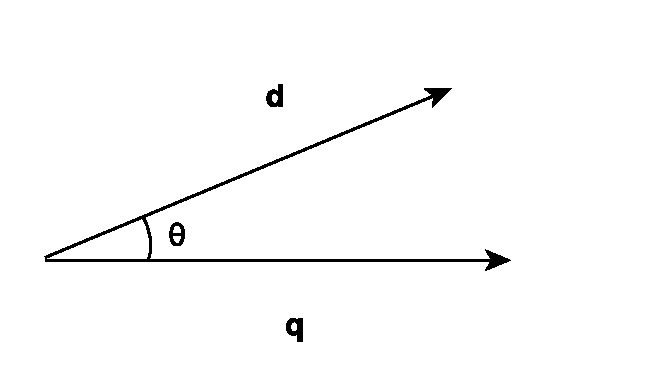
\includegraphics[scale = 0.6]{img/corner.pdf}}
		\caption{Косинусное сходство.}
		\label{fig2:image}
	\end{center}
\end{figure}

Косинусное сходство вычисляется по формуле (\ref{formula6}):
\begin{equation}\label{formula6}
	k_i = \frac{(\textbf{q}, \, \textbf{d}_i)}{\left| \textbf{q} \right| | \textbf{d}_i | }.
\end{equation}

Соответственно, чем значение ближе к 1, тем угол между векторами ближе к 0 градусам и два рассматриваемых вектора более схожи.

Таким образом, формируется множество 	$K = \, \left\lbrace k_1, ..., k_{|\tau|} \right\rbrace $. Наиболее подходящим под исходное описание считается тот термин, косинусное сходство которого является наибольшим в полученном множестве $K$.

Поскольку в рассматриваемой задаче все элементы любого из векторов являются неотрицательными (т.к. обозначают вес), то если $k_i = 0$, где  $i = \overline{1, |\tau|}$, это означает, что термины запроса отсутствуют в рассматриваемом документе. 

В отличие от метода шинглов такой подход не рассматривает информацию блоками, что, с одной стороны, лишает возможности проверки одновременного присутствия конкретных слов, но, с другой стороны, позволяет найти неточные совпадения лишь по части некоторых из них.\newline

\subsection{Семантические сети}
Кроме традиционного подхода в виде <<мешка слов>> для представления знаний используются семантические сети, которые строятся на графах.

Семантическая сеть -- ориентированный граф, в котором вершины соответствуют конкретным фактам, общим понятиям, объектам, а дуги -- отношениям или ассоциациям между ними \cite{network}.

Ассоциативному подходу уделяется особое внимание в силу того, что он описывает рассматриваемый объект в терминах его связей (по-другому, ассоциаций) с другими объектами. Ассоциации определяют, прежде всего, его свойства и поведение.\\
%
Объект может быть представлен как совокупность (рисунок \ref{fig3:image}), состоящая из:
\begin{itemize}
	\item характеристик и свойств;
	\item действий;
	\item набора состояний;
	\item множества объектов, так или иначе связанных с ним.
\end{itemize}

\begin{figure}[h]
	\begin{center}
		{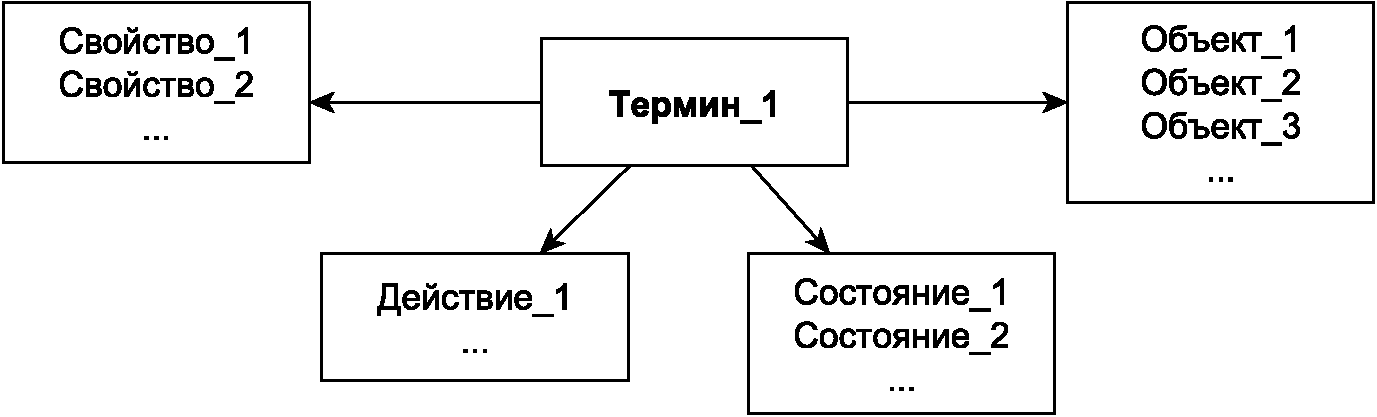
\includegraphics[scale = 0.6]{img/node.pdf}}
		\caption{Представление объекта при ассоциативном подходе.}
		\label{fig3:image}
	\end{center}
\end{figure}
%
Сеть строится из графов, и в случае совпадения узлов двух или более графов, они должны быть объединены и обновлены в соответствии с информацией, которая содержалась в узлах до их соединения. Пример простейшей сети представлен на рисунке \ref{fig4:image}.

\begin{figure}[h!]
	\begin{center}
		{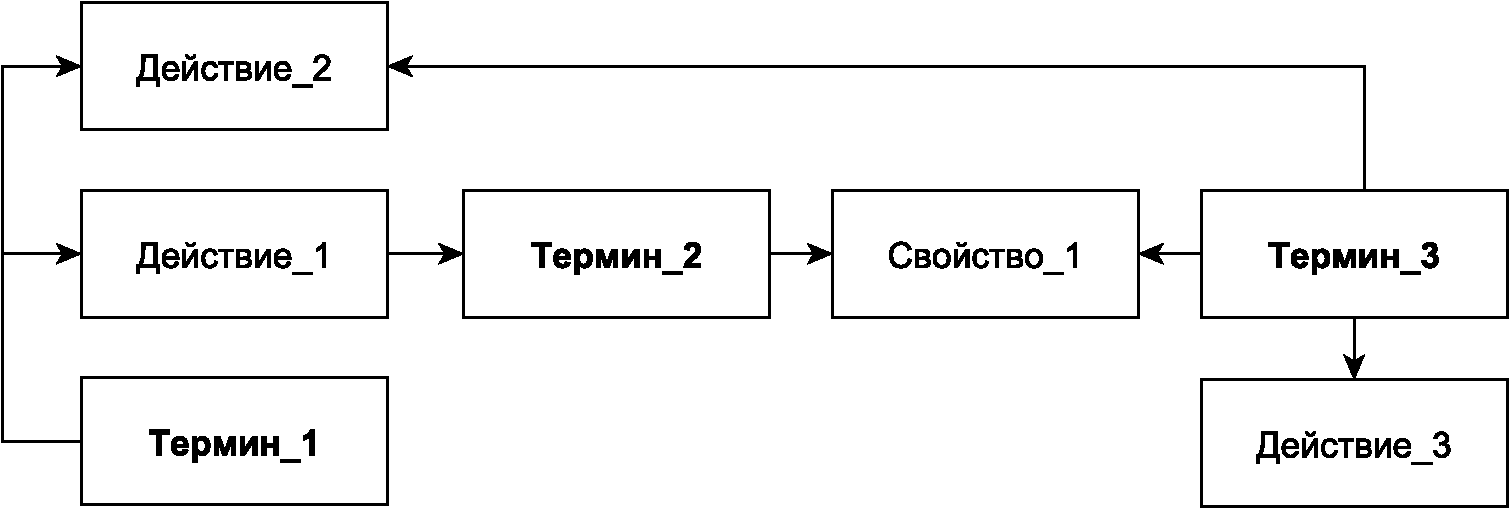
\includegraphics[scale = 0.6]{img/net.pdf}}
		\caption{Простейшая семантическая сеть.}
		\label{fig4:image}
	\end{center}
\end{figure}

\newpage

Термины 2 и 3 обладают одинаковым признаком <<Свойство 1>>, поэтому оба указывают на один узел, аналогичная \, ситуация наблюдается с \, <<Действием 2>>. \\

\subsection{Синтаксическое дерево}
Применимо к решаемой задаче, каждое предложение из онтологии может быть представлено в виде синтаксических деревьев, демонстрирующих связи между словами. Синтаксические единицы, как правило, изображаются в виде узлов, а связи -- дуг.

В синтаксическом дереве существует единственный узел, в который не входит ни одна дуга, и называется вершиной или корнем. Изображается он всегда сверху. Важной особенностью подобных структур является то, что в каждый узел (кроме корня) входит ровно одна дуга. 

В традиционной грамматике русского языка в качестве вершины предложения рассматривается подлежащее, в то время как в современной лингвистике корнем, как правило, считается сказуемое, от него напрямую или косвенно зависят все остальные члены предложения. Такой подход предложил французский лингвист Люcьен Теньер \cite{syntree}.

Согласно Теньеру, предложение -- <<драма в миниатюре>>, в центре которой находится действие. Вершина, глагол-сказуемое, называется предикатом, все остальные зависимые слова -- актанты (к ним относятся подлежащее, дополнения) и сирконстанты (обстоятельства). 

Одному предложению соответствует только одно синтаксическое дерево.

В Национальном корпусе русского языка \cite{examples} представлен синтаксический корпус объёмом около 1 миллиона примеров, оснащённых лингвистической разметкой, для каждого построено синтаксическое дерево, следуя принципам Теньера.

На рисунке \ref{fig5:image} представлено одно из них для предложения: <<Спрос на рынке труда постоянно меняется.>> \cite{exampleTree}.

\begin{figure}[h]
	\begin{center}
		{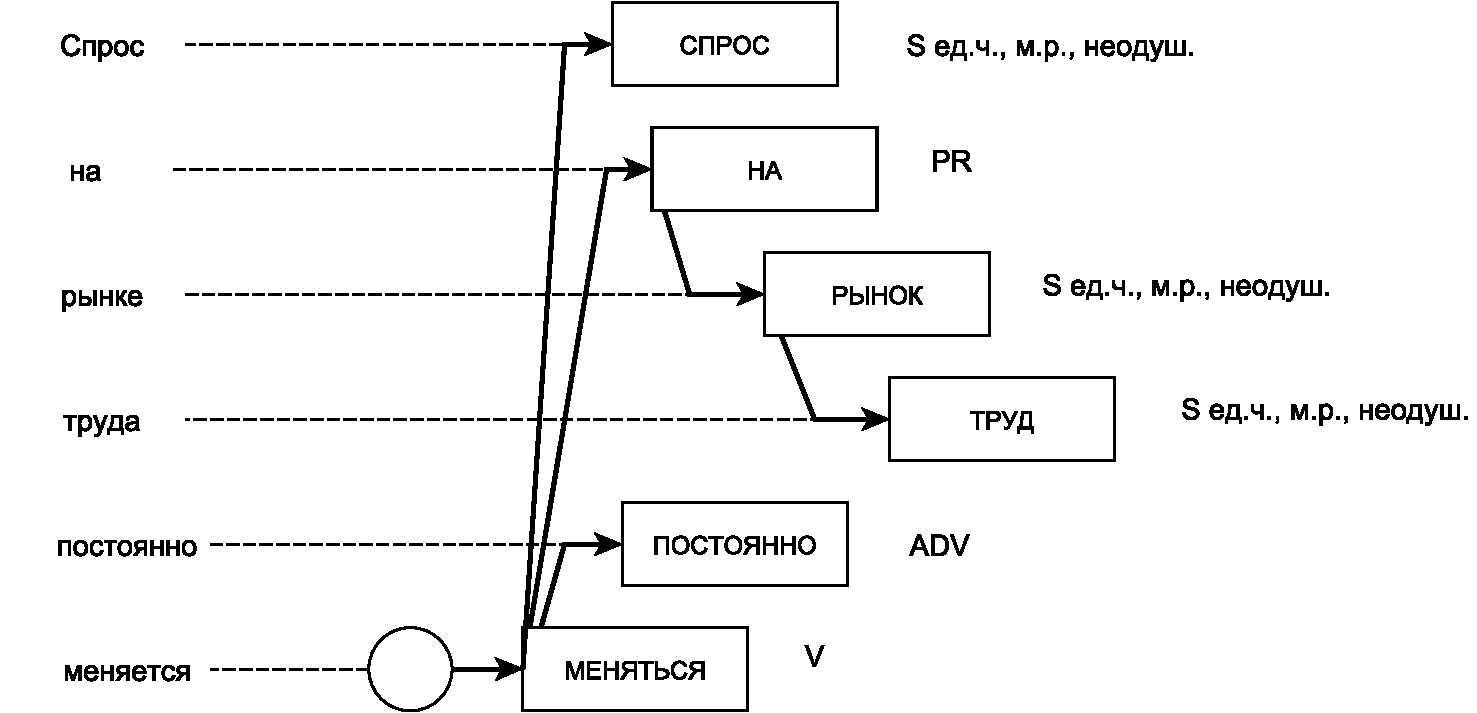
\includegraphics[scale = 0.6]{img/sentence.pdf}}
		\caption{Пример синтаксического дерева.}
		\label{fig5:image}
	\end{center}
\end{figure}

\subsection{Синтаксический граф}
Нередки случаи, когда одно и тоже слово в предложении повторяется, следовательно, в синтаксическом дереве будет создано несколько узлов, отведённых под один термин, но имеющих разных родителей. 

Во избежании дублирования информации и для упрощения процедуры составления семантической сети, лучше создавать по одному узлу на термин, но предусматривать возможность указания ему нескольких родителей. Из-за этого, в структуре данных могут возникать циклы. Следовательно, от формулировки <<синтаксическое дерево>> следует перейти к <<синтаксическому графу>>, так как первое не допускает наличие циклов. \\

\subsection*{Выводы}
Таким образом, в данной работе будет решаться задача определения объекта из ограниченной выборки терминов, касающихся двигателя внутреннего сгорания по его нечёткому описанию на русском языке. 

Были проанализированы существующие методы решения, выявлены основные преимущества и недостатки, среди которых невозможность некоторых из них работать с естественным языком и высокая стоимость. 

Также проанализированы основные алгоритмы работы с естественным языком, применимые к данной задаче. Был предложен способ её решения с помощью комбинации таких методов, как TF-IDF для формирования онтологии и сеть синтаксических графов в качестве вспомогательного метода, который будет привлекаться только в случае, если результаты обработки первым методом не будут удовлетворять критерию для принятия решения (степень уверенности меньше 50\%).

Также для поиска нечётких дубликатов между запросом пользователя и собранными заранее данными предлагается привлечение косинусного сходства.
\pagebreak